\documentclass[11pt]{paper}
\usepackage{fullpage}
\usepackage{booktabs}

% For rendering eps figures to pdf on different platforms. 
\ifx\pdftexversion\undefined
    \usepackage[dvips]{graphicx}
\else
    \usepackage[pdftex]{graphicx}
    \usepackage{epstopdf}
    \epstopdfsetup{suffix=}
\fi

\setlength{\tabcolsep}{5pt}

\begin{document}


%\phantom{0}
%\vspace{1.0in}
%
%
%\begin{centering}
%
%{\huge 
%Data Availability Guidelines and Code Base  \\
%\bigskip
%for \\
%\bigskip
%{\it ``Diversity Effects or Dissent Aversion? \\
%Identification and Estimation in Judicial Panel Voting''} \\
%}
%
%\vspace{1.25in}
%
%
%{\large 
%Charles M. Cameron \\
%{\it Center for the Study of Democratic Politics, Princeton University} \\
%\medskip
%Lealand Morin \\
%{\it College of Business, University of Central Florida} \\
%\medskip
%Harry J. Paarsch \\
%{\it College of Business, University of Central Florida} \\
%}
%
%\vspace{1.25in}
%
%
%
%\today
%
%\end{centering}

%\title[Penalties for Speeding and their Effect on Moving Violations]{Penalties for Speeding and their Effect on Moving Violations: Evidence from Quebec Drivers}
%
%\authors{V.~Chandler, L.~Morin, J.~Penney} 
%
%\authorone{Vincent Chandler}{Universit\'{e} du Qu\'{e}bec en Outaouais}
%
%\authortwo{Lealand Morin}{University of Central Florida} 
%
%\authorthree{Jeffrey Penney}{University of Alberta} 


% \pagebreak

\section*{Fixed Effects Regressions}


\begin{figure}
\centering
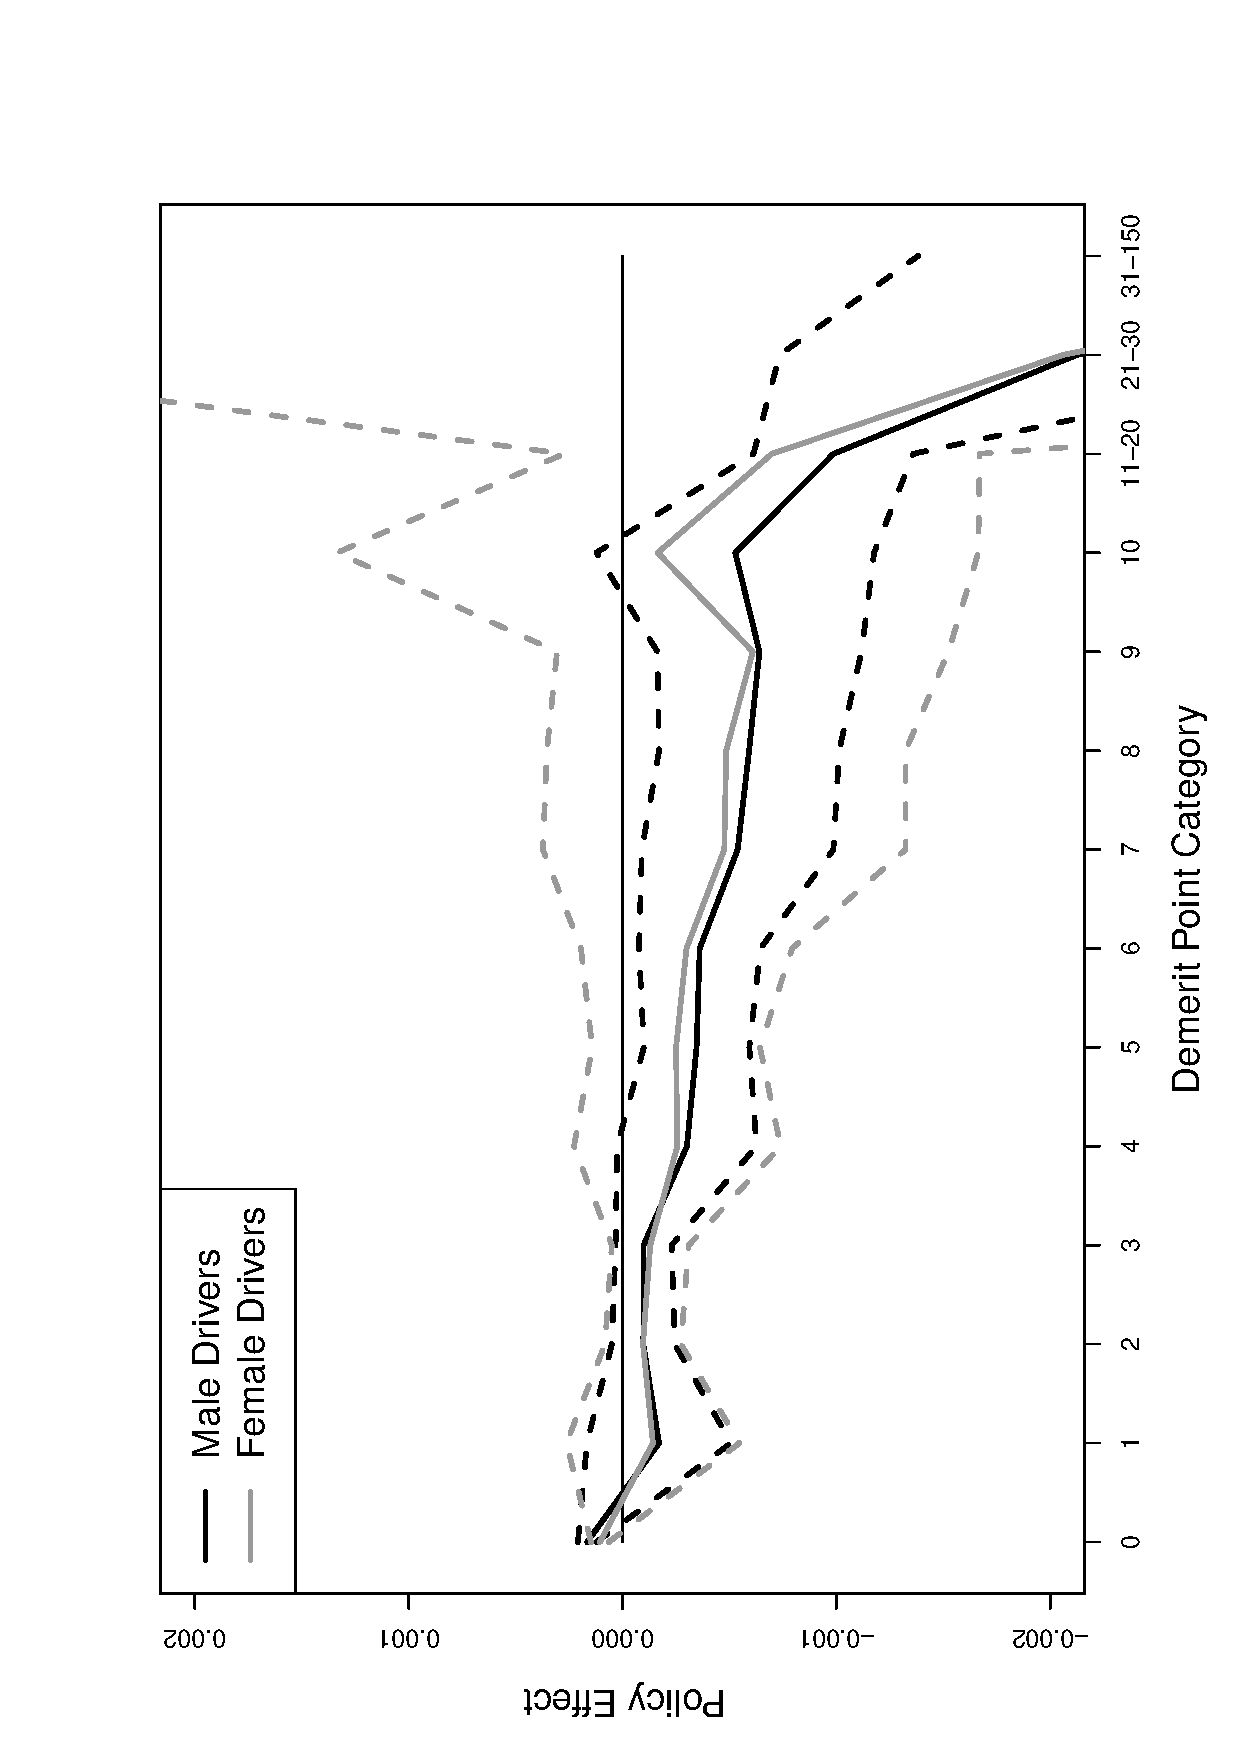
\includegraphics[width=0.8\textwidth]{../Figures/FFX_reg_policy_points_grp.pdf}
\caption{Policy change and demerit points group interactions}
%Coefficients on the interaction term between the change in the policy 
%by the current demerit points category of each driver.
%Estimates were calculated by fitting a fixed effects regression model, 
%with intercept coefficients for each driver. 
%% 
%Policy effects for male drivers are shown in black and those for females are shown in grey. 
%% 
%The dashed lines indicate upper and lower 95\% confidence intervals. }
% 
\label{fig:FE-regs}
\end{figure}


% Estimates from Fixed Effects Regression Models 

\begin{table}% [ht] 
\centering 
\begin{tabular}{l r r r r r r} 

\hline 
 

Sample 
 & \multicolumn{2}{c}{All  Drivers}  & \multicolumn{2}{c}{Male  Drivers}  & \multicolumn{2}{c}{Female  Drivers}   \\ 
 

 \cmidrule(lr){1-1}\cmidrule(lr){2-3}\cmidrule(lr){4-5}\cmidrule(lr){6-7} 

Estimate  & Coefficient & Std. Error  & Coefficient & Std. Error  & Coefficient & Std. Error   \\ 
 

\hline 
 
\multicolumn{4}{l}{\textbf{Demerit points group indicators:}}  \\ 
 
0 points  &  1.996  &  1.362  &  1.919  &  1.403  &  2.586  &  7.143   \\ 
 
1 points  &  1.422  &  1.365  &  1.412  &  1.409  &  1.918  &  7.145   \\ 
 
2 points  &  1.325  &  1.362  &  1.301  &  1.404  &  1.840  &  7.143   \\ 
 
3 points  &  1.325  &  1.362  &  1.290  &  1.403  &  1.855  &  7.143   \\ 
 
4 points  &  0.773  &  1.366  &  0.793  &  1.408  &  1.170  &  7.145   \\ 
 
5 points  &  0.764  &  1.364  &  0.779  &  1.406  &  1.154  &  7.144   \\ 
 
6 points  &  0.682  &  1.364  &  0.686  &  1.406  &  1.083  &  7.145   \\ 
 
7 points  &  0.301  &  1.370  &  0.332  &  1.413  &  0.577  &  7.151   \\ 
 
8 points  &  0.231  &  1.369  &  0.253  &  1.411  &  0.521  &  7.150   \\ 
 
9 points  &  0.293  &  1.370  &  0.257  &  1.414  &  0.850  &  7.151   \\ 
 
10 points  & -0.186  &  1.381  & -0.149  &  1.426  & -0.055  &  7.169   \\ 
 
11-20 points  & -0.537  &  1.366  & -0.521  &  1.408  & -0.323  &  7.150   \\ 
 
21-30 points  & -0.738  &  1.442  & -0.744  &  1.487  & -0.439  &  7.453   \\ 
 

\hline 
 
\multicolumn{4}{l}{\textbf{Policy and points group interactions:}}  \\ 
 
0 points  &  0.136  &  0.015  &  0.165  &  0.022  &  0.106  &  0.021   \\ 
 
1 points  & -0.160  &  0.132  & -0.171  &  0.172  & -0.142  &  0.206   \\ 
 
2 points  & -0.097  &  0.058  & -0.097  &  0.075  & -0.096  &  0.090   \\ 
 
3 points  & -0.108  &  0.054  & -0.099  &  0.067  & -0.130  &  0.092   \\ 
 
4 points  & -0.289  &  0.138  & -0.301  &  0.166  & -0.256  &  0.246   \\ 
 
5 points  & -0.321  &  0.106  & -0.346  &  0.126  & -0.250  &  0.200   \\ 
 
6 points  & -0.346  &  0.125  & -0.361  &  0.145  & -0.299  &  0.252   \\ 
 
7 points  & -0.530  &  0.201  & -0.538  &  0.228  & -0.476  &  0.433   \\ 
 
8 points  & -0.573  &  0.191  & -0.592  &  0.215  & -0.485  &  0.428   \\ 
 
9 points  & -0.631  &  0.215  & -0.640  &  0.243  & -0.609  &  0.467   \\ 
 
10 points  & -0.475  &  0.302  & -0.527  &  0.331  & -0.165  &  0.765   \\ 
 
11-20 points  & -0.950  &  0.177  & -0.986  &  0.191  & -0.698  &  0.496   \\ 
 
21-30 points  & -2.119  &  0.683  & -2.125  &  0.709  & -2.061  &  2.982   \\ 
 
31-150 points  & -4.520  &  1.555  & -4.524  &  1.603  & -4.378  &  8.025   \\ 
 

\hline 
 

Drivers 
 & \multicolumn{2}{r}{1,694,022}  & \multicolumn{2}{r}{1,093,342}  & \multicolumn{2}{r}{600,681}   \\ 
 

Driver days 
 & \multicolumn{2}{r}{5,589,577,894}  & \multicolumn{2}{r}{3,042,464,204}  & \multicolumn{2}{r}{2,547,113,690}   \\ 
 

SSR 
 & \multicolumn{2}{r}{7,451,089}  & \multicolumn{2}{r}{5,054,882}  & \multicolumn{2}{r}{2,311,376}   \\ 
 

\hline 
 
\end{tabular} 
\caption{Estimates from Fixed Effects Regression Models} 
Fixed effects regression coefficients after estimating driver-specific intercepts.. 
Samples are drawn by selecting 40 per cent of the drivers in each sample. 
\label{FE_regs} 
\end{table} 
 




\end{document}
